\documentclass[10pt,twocolumn]{article}

\usepackage[margin=0.85in]{geometry}
\usepackage{amsmath}
\usepackage{amssymb}
\usepackage{booktabs}
\usepackage{graphicx}
\usepackage{array}
\usepackage[hidelinks]{hyperref}
\usepackage{xcolor}

\newcommand{\todo}[1]{\textcolor{red}{[#1]}}

\title{\textbf{Learned and Classical Control on a Rocket\\ Soft-Landing Task, and Bidirectional\\ Knowledge Transfer Between Them}}
\author{Aditya Anil Shukla\\ \small University of London, CM3070 Final Project}
\date{Draft v0.1, \today}

\begin{document}
\maketitle

\begin{abstract}
We study soft-landing control of a simulated rocket booster that must touch down upright and gently on a narrow pad from a wide distribution of initial offsets, lateral velocities, and spins. On a modern, reproducible rebuild of an earlier project (Gymnasium, Stable-Baselines3, seeded evaluation, continuous integration), we compare an on-policy reinforcement learning agent (PPO), an off-policy agent (SAC), and two hand-designed classical controllers. At full difficulty, PPO lands about 91\% of episodes, essentially matching a careful classical controller (about 89\%), while landing roughly 2.6 times faster on near-zero thruster fuel because the reward values time and fuel. We then study knowledge transfer in both directions. From learned to classical: we distill PPO's fast ``hoverslam'' strategy into a two-parameter braking profile and implement it in a deterministic controller that lands about 86 to 90\% at roughly half the time of the careful controller, and smoother, which establishes a measured Pareto ceiling where fast-and-reliable-everywhere is not reachable by hand at the continuous actuator's slew rate. From classical to learned: we seed SAC with controller demonstrations, which breaks SAC's zero-landing floor; the demonstration-induced landings first erode under a ``discount dilemma'' between a hover attractor and a crash attractor, until a potential-based descent-profile shaping term reshapes the value landscape and makes them persist, lifting SAC to about 70\% (from 0\%), still below PPO and the classical controllers. We report honest measurement caveats throughout and argue that the limitations are themselves part of the contribution.
\end{abstract}

\section{Introduction}

Rocket booster recovery is a hard precision control problem: the vehicle must arrive at a small target, upright, below a strict touchdown speed, from adverse initial conditions, under tight fuel and time pressure. It is a natural testbed for comparing learned control (reinforcement learning, RL) against classical feedback control, and for studying whether insight can be transferred between the two paradigms.

This paper makes the following contributions.
\begin{itemize}
  \item A faithful, reproducible modern rebuild of a rocket soft-landing study, on which an on-policy RL agent (PPO) reaches about 91\% landing at full difficulty, reproducing the earlier result on a seeded, continuous-integration-backed pipeline.
  \item A head-to-head comparison showing that learned and well-designed classical control reach near parity on landing reliability, while the learned agent is far more time- and fuel-efficient because the reward rewards efficiency.
  \item A learned-to-classical distillation: PPO's fast landing strategy is reduced to a two-parameter braking profile and implemented in a deterministic controller that flies the learned strategy by hand, with a measured Pareto ceiling attributable to actuator-speed asymmetry.
  \item A classical-to-learned transfer study (demonstration-seeded SAC) that breaks the agent's zero-landing floor but does not stabilize it within budget, together with a mechanistic account (the discount dilemma) of why.
  \item An emphasis on honest measurement: best-checkpoint selection on a disjoint seed bank, held-out confirmation banks, and an explicit statement of the discrete-versus-continuous action-space confound.
\end{itemize}

\section{Related Work}

Deep RL has been applied widely to continuous control. Proximal Policy Optimization (PPO) \cite{schulman2017ppo} is a stable on-policy policy-gradient method; Soft Actor-Critic (SAC) \cite{haarnoja2018sac} is an off-policy maximum-entropy actor-critic that is typically more sample-efficient on dense-reward continuous-control benchmarks. Classical feedback control (cascaded loops, feedback linearization, gain scheduling) remains the standard for aerospace guidance and is strong when a model is available.

Learning from demonstrations and policy distillation seek to transfer behavior from an expert into a policy. DDPGfD \cite{vecerik2017ddpgfd} seeds an off-policy replay buffer with demonstrations and adds an auxiliary behavior-cloning loss; imitation learning is surveyed in \cite{hussein2017imitation}. Potential-based reward shaping \cite{ng1999shaping} adds a shaping term of the form $\gamma\Phi(s')-\Phi(s)$ that provably preserves the optimal policy while reshaping the value landscape. Our classical-to-learned study combines these ideas. We keep citations modest and verifiable; where we were unsure of a precise reference we omitted it rather than fabricate one.

\section{Environment and Task}

\paragraph{Simulator.} The environment is a Box2D rigid-body model of a booster descending toward a landing pad, exposed through the Gymnasium interface. The vehicle starts near the top of the world falling at a scaled speed of 80, and must land on a pad that is narrow relative to the lateral spread of the initial conditions.

\paragraph{Observation.} The 10-dimensional observation contains horizontal and vertical position relative to the pad, body angle, two landing-leg ground-contact flags, current throttle and engine gimbal, and the three velocity components.

\paragraph{Actions.} The continuous action space is a 3-vector in $[-1,1]^3$: an engine gimbal rate, a throttle rate, and a side (reaction-control) thruster that is effectively ternary. A discrete action space of 7 actions (gimbal and throttle increments, side thrusters, no-op) is also available and is what the original PPO agent used. The main engine has a minimum-throttle floor: once lit, it produces at least 40\% thrust, so the vehicle cannot throttle far below its own weight.

\paragraph{Reward.} The per-step reward combines a potential-based shaping term on distance, speed, and angle, a small fuel cost, a per-step cost while airborne, a sparse $+1$ bonus for a sustained soft landing, and a terminal penalty for crashing or leaving the frame. The per-step reward is clipped to $[-1,1]$.

\paragraph{Landing criterion.} A landing requires both legs in ground contact and a settled speed below a fixed gate, sustained for a short window. Episodes run to a 3000-step cap, which is important: a successful careful descent can take on the order of 1000 to 2000 steps, so a shorter cap truncates exactly the trajectories through which landing is discovered.

\paragraph{Difficulty.} At full difficulty the initial lateral offset spans up to about $\pm0.3$ of the world width (several pad widths), with randomized initial horizontal velocity and spin up to about $\pm1.4$ rad/s. An eased variant halves these; we report full difficulty throughout except where stated.

\paragraph{Reproducible rebuild.} The study was rebuilt on a modern stack (Gymnasium, Stable-Baselines3, PyTorch) managed with \texttt{uv}, with a dataclass-based configuration system, per-environment monitoring, a seeded paired evaluation harness, and continuous integration. A bit-level differential test against the original environment (identical seeded initial conditions and action sequence) found the reward identical to within floating-point rounding and the observations identical up to a float32 cast, so the rebuilt task is the same task.

\section{Methods}

\subsection{Reinforcement learning agents}
PPO is trained on the discrete action space with static observation normalization, 16 parallel environments, a small learning rate, and few epochs, to roughly 15 to 20 million environment steps. SAC is trained on the continuous action space with static observation normalization and a single or small number of environments.

\subsection{Classical controllers}
We implement two cascaded, feedback-linearized controllers that share inner attitude, gimbal, throttle, and reaction-control loops.
\begin{itemize}
  \item \textbf{Careful controller.} A patient glide-slope descent that brakes to near-hover early, then descends slowly while continuously centering over the pad. It is reliable but slow (about 22 s).
  \item \textbf{Fast controller (PPO-distilled).} See Section~\ref{sec:distill}. It flies a constant-deceleration braking profile with time-to-go-scheduled lateral gates and a latched fast/patient router that diverts the hardest entries to the careful path.
\end{itemize}
Both controllers cut the main engine once both legs are planted so the vehicle seats and settles, matching real boosters.

\subsection{Distilling PPO into a deterministic controller}
\label{sec:distill}
We probe the trained PPO policy over many landings and quantify its strategy, then reduce it to a small number of control constants. PPO lights the engine immediately and brakes at a nearly constant deceleration of about 8 m/s$^2$ the whole way down (a ``hoverslam''), arriving at the pad at the edge of leg survivability, steering almost entirely by gimbal-induced body tilt rather than the reaction-control thrusters. The distilled vertical reference is
\begin{equation}
v_{\mathrm{ref}}(h) = -\min\!\big(V_{\mathrm{TD}} + K\,h,\ \sqrt{V_{\mathrm{TD}}^2 + 2\,A\,h}\big),
\end{equation}
with a touchdown-speed target $V_{\mathrm{TD}}$ and a braking deceleration $A$. This two-parameter curve captures essentially all of PPO's time advantage.

\subsection{Demonstration-seeded SAC}
To address SAC's failure to discover the sparse landing (Section~\ref{sec:sac}), we seed its replay buffer with demonstrations from the continuous fast controller (which lives in SAC's exact action space, unlike the discrete PPO). We use a reserved demonstration partition mixed into every minibatch, an auxiliary behavior-cloning (BC) loss on the demonstration actions, and a potential-based descent-profile shaping term $\Phi(s) = -w\,|v_y - v_{\mathrm{ref}}(h)|$ applied as $\gamma\Phi(s')-\Phi(s)$ to remain policy-invariant.

\section{Experimental Setup}

Evaluation uses a seeded, paired protocol: every controller is run on an identical bank of held-out initial conditions, with RL policies evaluated deterministically. We select the best training checkpoint on one seed bank and report on a disjoint bank, and we additionally confirm on further fresh banks to rule out seed-specific selection bias. We report landing rate with Wilson score intervals and continuous metrics with bootstrap intervals, and we use McNemar and Wilcoxon signed-rank tests for paired comparisons.

A hardware note frames the RL comparison: PPO trains at roughly 11{,}000 environment steps per second (16 CPU environments with a tiny policy network), whereas SAC trains at roughly 280 steps per second (a single environment with a per-step GPU gradient update), about 40 times slower in wall-clock per environment step.

\section{Results}

\subsection{Main comparison}
Table~\ref{tab:main} reports the main results at full difficulty on the held-out bank. PPO and the careful classical controller reach near parity on landing rate. The fast distilled controller matches that reliability at roughly half the time and lower fuel. SAC trails substantially at its baseline.

\begin{table}[t]
\centering
\caption{Landing performance at full difficulty (3000-step cap, seeded held-out banks, deterministic policies). Smoothness is mean $|\Delta a|$ per step; not comparable across the discrete/continuous boundary.}
\label{tab:main}
\small
\begin{tabular}{@{}lcccc@{}}
\toprule
Controller & Landing & Time & Fuel & Smooth. \\
\midrule
PPO (on-policy)        & $\sim$91\% & $\sim$9 s  & $\sim$0.00 & n/a \\
Classical, careful     & $\sim$89\% & $\sim$22 s & $\sim$1.0  & 0.26 \\
Classical, fast        & 86--90\%   & $\sim$11 s & $\sim$0.6  & 0.24 \\
SAC (vanilla)          & 0\%        & --         & --         & -- \\
SAC (demo-seeded)      & $\sim$70\% & $\sim$19 s & $\sim$0.6  & smooth \\
\bottomrule
\end{tabular}
\end{table}

\subsection{Reproduction and no overfitting}
PPO's performance is checkpoint-dependent: its 15M-step checkpoint lands 91\% while the final 20M model degrades to about 76\% as the policy oscillates late in training (hence best-checkpoint selection). Evaluated on two further fresh seed banks never used for selection, the 15M checkpoint lands 91\% and 88\%, so the headline number generalizes and is not an artifact of the seeds it was tuned on. We also note that the original project's 91\% was measured with a stochastic policy, a cherry-picked checkpoint, and stdout-string success detection, whereas ours is deterministic, seeded, and based on the ground-truth landing flag; the success criterion itself is identical.

\subsection{Efficiency}
On a matched easy-mode bank where both land 100\%, the median time-to-land is 8.9 s for PPO versus 22.9 s for the careful controller, a factor of 2.6, and PPO uses essentially zero reaction-control fuel (0.00 versus 0.43). PPO is efficient because the reward charges for time airborne and for fuel; the careful controller, tuned only for reliability, trades both away. This also connects to physical realism: a real booster cannot hover (its minimum thrust exceeds its weight), so it must perform a fast committed hoverslam, which is closer to PPO's behavior than to the careful controller's slow hover-crawl.

\subsection{Learned-to-classical distillation}
The distilled fast controller lands 86 to 90\% across held-out banks (versus 82 to 92\% for the careful controller, within sampling noise), at a median of about 11 s (versus 22 s) and lower fuel, while being at least as smooth. The fast landing strategy therefore transfers cleanly, because it is a trajectory property captured by two constants. What does not transfer is the last increment of reliability. A dedicated sweep found a Pareto ceiling of about 86 to 87\%: 90\% at fast speed is not reachable by hand. The dominant cause is actuator asymmetry. PPO's discrete interface moves the gimbal about 40 times faster per step than the continuous interface's slew limit, so on the hardest off-center entries PPO can reverse the body tilt in a fraction of the time available while the hand-coded controller cannot. The remaining failures are almost entirely soft, upright touchdowns that land just outside the narrow pad, a lateral-precision limit, plus a few single-leg tip-overs; essentially none are high-speed impacts.

\subsection{Classical-to-learned transfer and the discount dilemma}
\label{sec:sac}
SAC does not discover the landing by exploration. At discount $\gamma=0.99$ it falls into a hover attractor (the discounted cost of hovering is smaller than that of crashing, and the distant landing bonus is discounted to near zero), spending 20 to 30\% of its budget hovering. Raising the discount to $\gamma=0.997$ removes hovering but produces a crash attractor: episodes become short dive-to-crash trajectories, with zero landings across more than a million steps. The task itself is landable (PPO lands it under the same reward), so this is an exploration-and-optimization failure specific to off-policy SAC on this geometry.

Seeding demonstrations addresses exploration but introduces new pathologies. Naive replay seeding diverges the critic (value estimates grow by orders of magnitude, from order one to roughly $+4000$) because the policy never reaches the near-pad demonstration states and the bootstrap there goes uncorrected. Adding a behavior-cloning auxiliary loss bounds the critic completely. With strong behavior cloning, landings appear and are dose-responsive to the cloning strength (zero, zero, three, then fourteen landings as the coefficient increases), and these are genuine soft landings. However, the landings erode: in every run they appear in the first half of training and then vanish as the value gradient pulls the actor back off the demonstration manifold. We therefore characterize the obstacle as a discount dilemma: both discount settings carry a pathological attractor, and a behavior-cloning constraint on actions cannot reshape the value landscape that produces the attractor. The principled remaining lever is potential-based descent-profile shaping, which reshapes the value landscape while remaining policy-invariant. This resolves the erosion. With the shaping term at $w=0.3$, landings persist into the second half of training, and a dose-response isolates shaping as the cause: $w=0$ and $w=0.1$ both erode, while $w=0.3$ sustains a landed fraction near 0.4 with the critic bounded throughout. Because the shaping is policy-invariant, the solve is genuine rather than a shaping artifact. Evaluated deterministically on the unshaped environment over the standard held-out banks, the best checkpoint lands about 70\% (up from 0\% for vanilla SAC and about 48\% for the tuned baseline), with soft touchdowns near 0.004. The landing policy peaks early and erodes if trained too long, so we report the best checkpoint rather than the final one. SAC still trails PPO (about 91\%) and the classical controllers (about 86 to 90\%).

\subsection{Robustness to distribution shift}
\label{sec:robust}
All reported figures so far are in-distribution. To test generalization, we perturb the evaluation environment in ways no controller trained or was tuned for, applying each perturbation identically to every controller on a shared 30-seed bank. The outcomes separate the methods sharply and in opposite ways depending on the perturbation.

Under \emph{observation noise} (zero-mean Gaussian added in the normalized observation space, Figure~\ref{fig:robust}, left), the learned agents are far more robust than the hand-coded controllers. PPO holds at 93 to 97\% across all noise levels and SAC holds near 70\% until the largest, while both classical controllers collapse from about 83\% to near zero by a noise standard deviation of 0.1. A learned policy is a smooth function of its observation and tolerates corruption; the classical controllers decode noisy state into saturated feedback and tip over. Under \emph{wind} (a constant lateral force) and \emph{wider initial conditions}, all methods degrade and PPO is generally the most robust, though no method survives the strongest wind.

\emph{Vehicle mass mismatch} (Figure~\ref{fig:robust}, right) exposes an instructive asymmetry. PPO is near-perfect when the booster is lighter than nominal (100\% at $0.9\times$) but collapses when it is heavier (30\% at $1.1\times$, 0\% at $1.15\times$). The classical controllers are the mirror image: they fail when the booster is lighter (0\% at $0.9\times$) because their feedback-linearized thrust uses a fixed mass constant, yet they tolerate a heavier booster better than PPO. Neither paradigm was exposed to mass variation, and each is sensitive in the direction its fixed assumption (a learned thrust response, or a hard-coded mass) does not cover. Full tables and figures for all four perturbations are in the repository.

\begin{figure}[t]
\centering
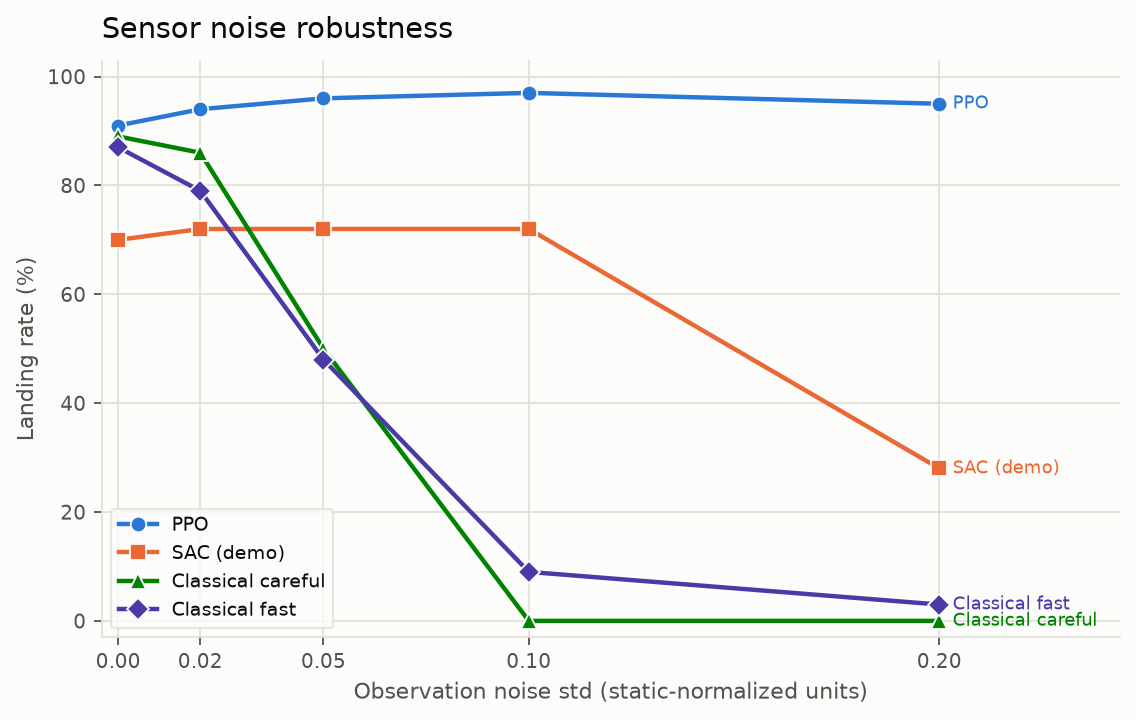
\includegraphics[width=0.49\linewidth]{../assets/robustness/robustness_sensor_noise.png}
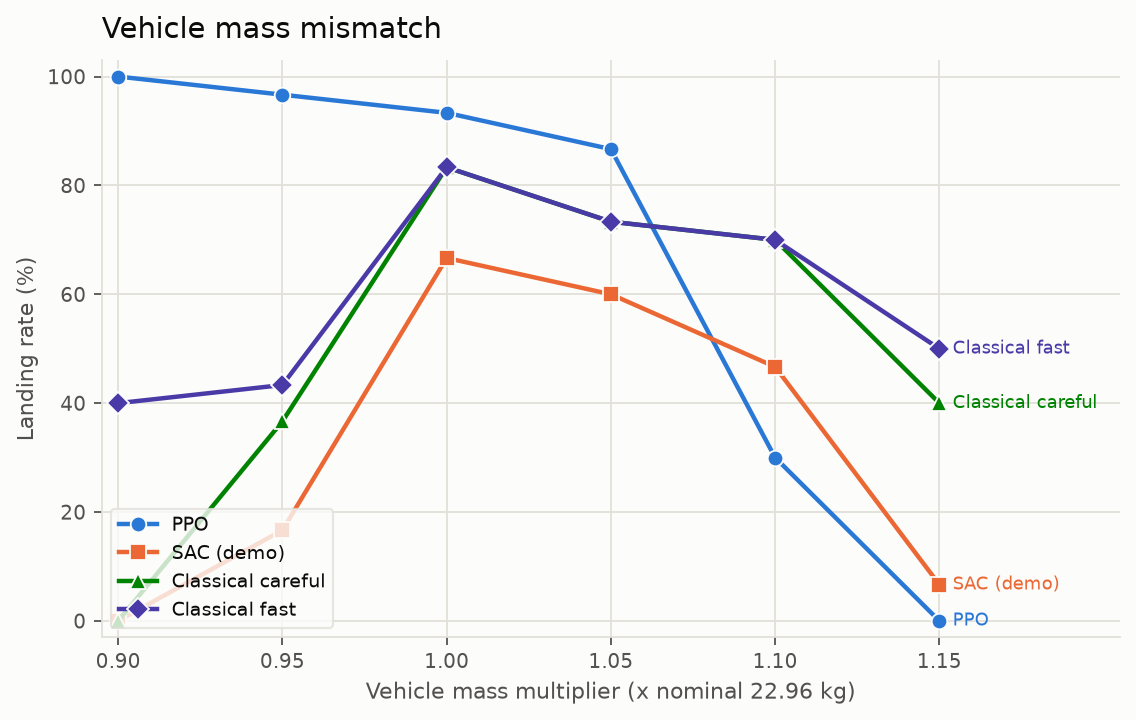
\includegraphics[width=0.49\linewidth]{../assets/robustness/robustness_mass.png}
\caption{Robustness to distribution shift. Left: observation noise, where learned agents degrade gracefully and classical controllers collapse. Right: vehicle mass mismatch, where PPO and the classical controllers fail in opposite directions. Landing rate over 30 shared seeds.}
\label{fig:robust}
\end{figure}

\section{Discussion}

Several findings stand out. First, the study reproduces the earlier learned-control result on a modern, seeded, reproducible pipeline, and a bit-level test confirms the environment is faithful. Second, learned and well-designed classical control reach near parity on reliability on this hard precision task, rather than one paradigm dominating. Third, the learned agent's efficiency is a direct consequence of reward design, not of the learning paradigm per se. Fourth, learned-to-classical distillation works for the parts of behavior that are trajectory properties (speed and smoothness) but not for the parts that are actuator properties (the fast-and-reliable frontier), which gives a clean, measured answer to whether a deterministic controller can be improved from RL findings: partially, with a nameable ceiling. Fifth, classical-to-learned transfer is harder here, because demonstrations constrain actions rather than the value function, and the value function is where the pathology lives.

\section{Limitations}

The study is simulation-only, so sim-to-real transfer is untested and the agents may exploit simulator quirks. Several headline numbers come from a single training seed; multi-seed runs with confidence intervals are future work. The PPO-versus-SAC comparison is confounded by action space (PPO is discrete, SAC continuous); the 89\% of the classical controllers through the same continuous interface shows the interface can support about 90\%, so the interface is not the explanation, but the comparison is not strictly apples-to-apples and we state it plainly. The initial-condition difficulty, the touchdown-speed gate, and the landing-tick window are task-shaping choices; we report full difficulty but acknowledge they are knobs.

\section{Conclusion and Future Work}

On a rocket soft-landing task, on-policy PPO and principled classical control reach near-parity reliability, with PPO far more efficient; the RL agent's fast strategy distills cleanly into a deterministic controller up to an actuator-limited ceiling; and seeding demonstrations into off-policy SAC breaks its zero-landing floor while a potential-based descent-profile shaping term stabilizes it to about 70\%, still below the other methods, with the obstacle traced to a discount dilemma. A robustness study (Section~\ref{sec:robust}) shows learned agents are much more tolerant of observation noise than the classical controllers, while mass mismatch breaks the two paradigms in opposite directions. Future work includes domain-randomized training to close those robustness gaps, more training seeds for tighter confidence intervals, and raising the minimum-throttle floor so the task becomes genuinely hoverslam-only and closer to a real booster.

\begin{thebibliography}{9}
\small
\bibitem{schulman2017ppo} J. Schulman, F. Wolski, P. Dhariwal, A. Radford, O. Klimov. Proximal Policy Optimization Algorithms. arXiv:1707.06347, 2017.
\bibitem{haarnoja2018sac} T. Haarnoja, A. Zhou, P. Abbeel, S. Levine. Soft Actor-Critic: Off-Policy Maximum Entropy Deep Reinforcement Learning with a Stochastic Actor. ICML, 2018.
\bibitem{ng1999shaping} A. Y. Ng, D. Harada, S. Russell. Policy Invariance Under Reward Transformations: Theory and Application to Reward Shaping. ICML, 1999.
\bibitem{vecerik2017ddpgfd} M. Vecerik et al. Leveraging Demonstrations for Deep Reinforcement Learning on Robotics Problems with Sparse Rewards. arXiv:1707.08817, 2017.
\bibitem{hussein2017imitation} A. Hussein, M. M. Gaber, E. Elyan, C. Jayne. Imitation Learning: A Survey of Learning Methods. ACM Computing Surveys, 2017.
\end{thebibliography}

\end{document}
